% Bending about the y-axis: w(x) and w'(x) > 0
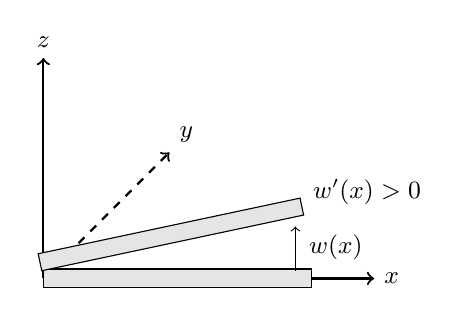
\begin{tikzpicture}[scale=1.0,font=\small]
  \draw[->,thick] (0,0) -- (4.2,0) node[right] {$x$};
  \draw[->,thick] (0,0) -- (0,2.8) node[above] {$z$};
  \draw[->,thick,dashed] (0,0) -- (1.6,1.6) node[above right] {$y$};
  \draw[fill=black!10] (0,-0.12) rectangle (3.4,0.12);
  \draw[fill=black!10,rotate=12] (0,0.1) rectangle (3.4,0.32);
  \draw[->] (3.2,0.1) -- (3.2,0.66); \node[right] at (3.25,0.4) {$w(x)$};
  \node[right] at (3.3,1.1) {$w'(x)>0$};
\end{tikzpicture}
